\documentclass[../main.tex]{subfiles}
\graphicspath{{\subfix{../images/}}}
\begin{document}

(Translated passage from Anatomie--Atlas~\cite{AAtlas})
\section{Voyage Through the Body}

Olfactory cells detect the roast, they locate toasted compounds, the marjoram and so on.
They stimulate the flow of the juices into the mouth, get you excited for the first bite.
In the hypothalamus\index{hypothalamus} (figure~\ref{hypothalamus}) in the brain is the seat of the central of the appetite, which directs all the processes.
It gets information from the body about how high the blood sugar levels are, from the fat cell if they need replenishment.
That is the seat of the somatic intelligence (body--centered intelligence)\index{somatic intelligence}.
The ancient knowledge of the body, which knows what the body needs.
Unfortunately, that part of us is asleep in most of us.
It should coordinate hunger, cravings and satiation; we move a lot, we need a lot of calories.
The hypothalamus directs a whole army of hunger--saturation hormones\footnote{Almost weekly science discovers a new one.}.\index{hormones!hunger--satiation}
Either it's 'eat more', or if we have a sedentary period it switches to the energy save program --- satiation sets in earlier.
This ancient wisdom urges us with craving of lemons, if the immune system needs a vitamin C boost or a craving for cheese if the bones needs calcium.
The problem is that we suppressed this ancient wisdom because we're not eating anymore due to being hungry but due to what time dictates.
It is suppressed because we're not eating anymore what he body needs but empty calories, jazzed up with artificial aromas.
The head says, 'I want apple pie'. But that's not what the body says, the apple pie isn't good for it. It'd prefer the apple by itself.
That's what in the genetic program, that what fits with the metabolism.

\begin{figure}[h]
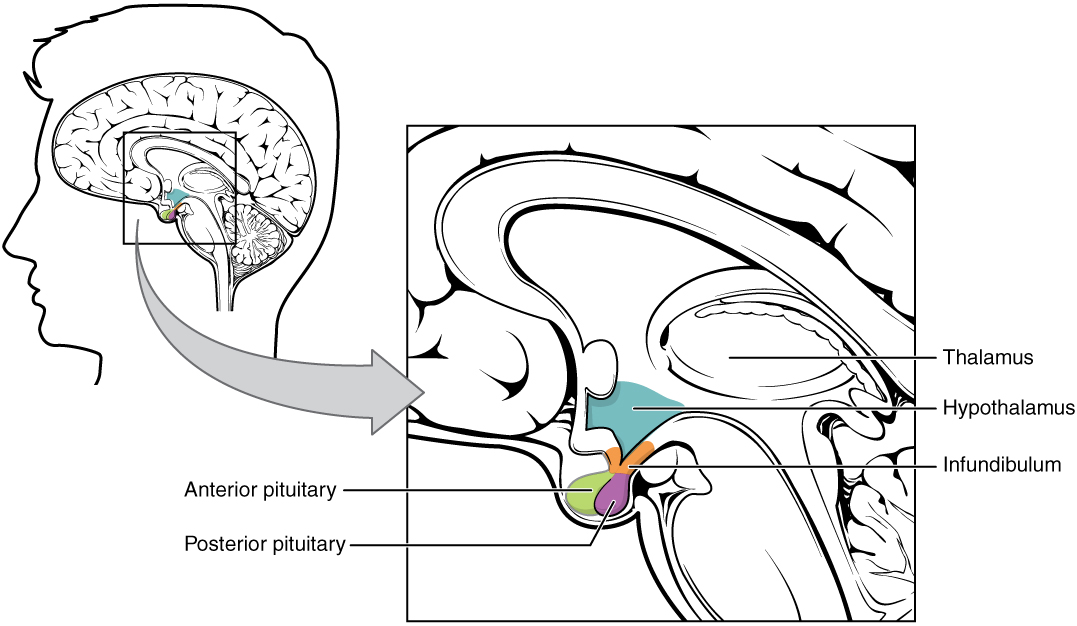
\includegraphics[width=12.5cm]{Hypothalamus}
  \caption{The hypothalamus~\cite{hypothalamus} and~\cite{hypothalamus-detail}}\label{hypothalamus}
\end{figure}



\begin{figure}[htb!]
  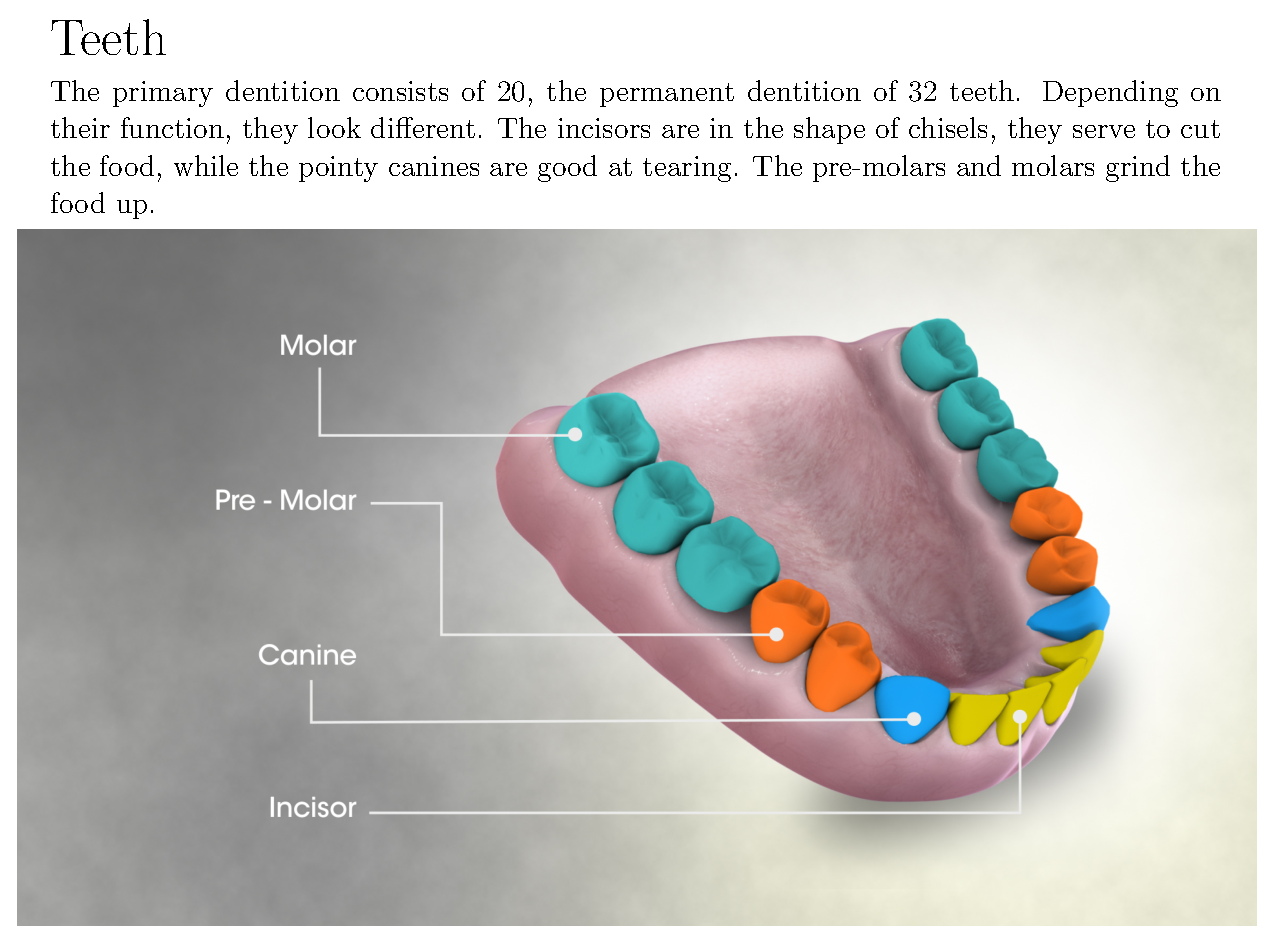
\includegraphics[width=12.5cm]{Teeth}
  \caption{The human teeth~\cite{SciAnim}}\label{teeth}
\end{figure}

\begin{figure}[htb!]
  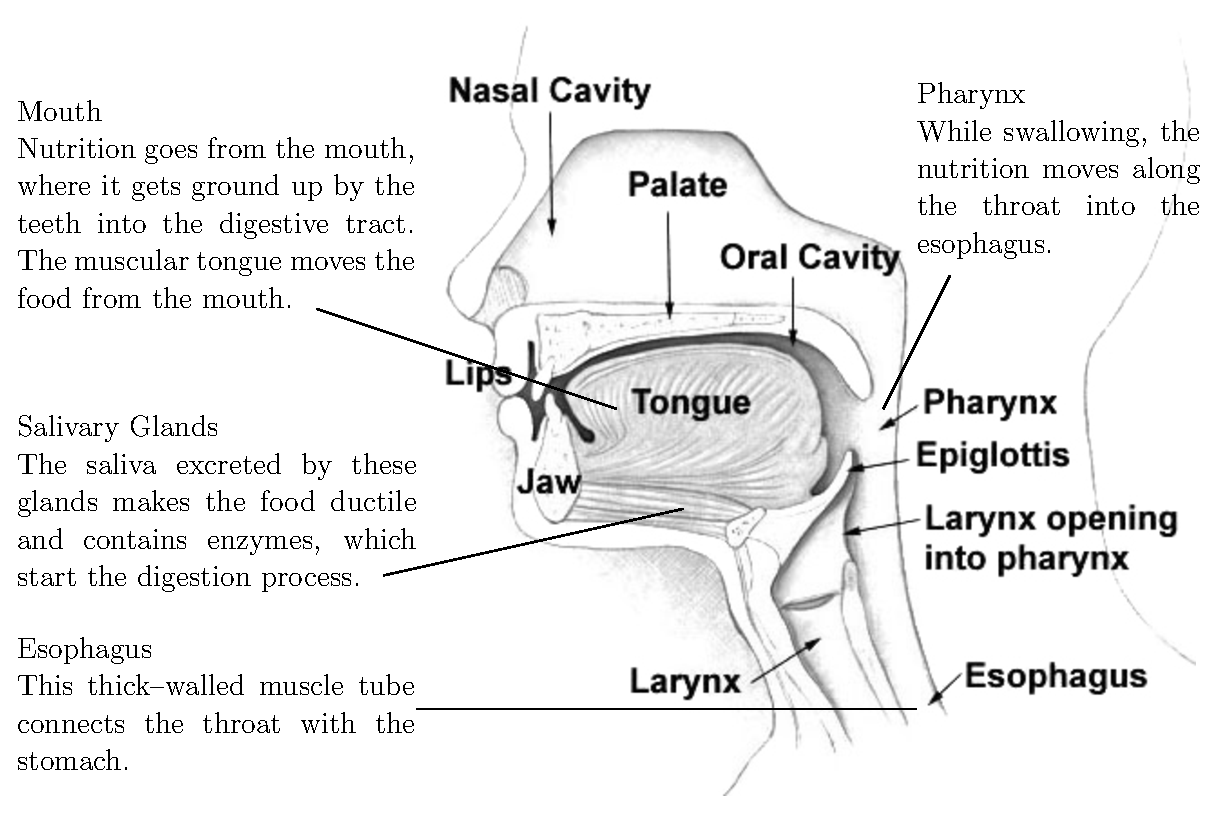
\includegraphics[width=12.5cm]{Mouth}
  \caption{The human mouth and esophagus~\cite{Mouth}}\label{mouth}
\end{figure}

  The hypothalamus in the brain, the central of appetite registers how much fat is in the fat cells and how much sugar in the blood.
If it finds something missing, it triggers hunger.

\section{The Miracle of the Digestion}

You eat pasta with veggies and shrimp.
A chemist would say: carbohydrates\index{carbohydrates}, fibers, vitamins, minerals, fat and proteins\index{proteins}.
Already in the mouth (see teeth, picture \ref{teeth})\index{digestion}
will the saliva\index{saliva} (salivary gland, picture \ref{mouth}) cleave carbohydrates, with it's enzymes.
The longer you chew it, the sweeter will the pasta be.
The long carbohydrate chains of the starch\index{starch} gets cleaved into small sugar molecules\index{sugar}.
Chewing grinds up the food, and increases the surface area and therefore the exposure to the digestive tools of the body. 


\begin{figure}[htb!]
  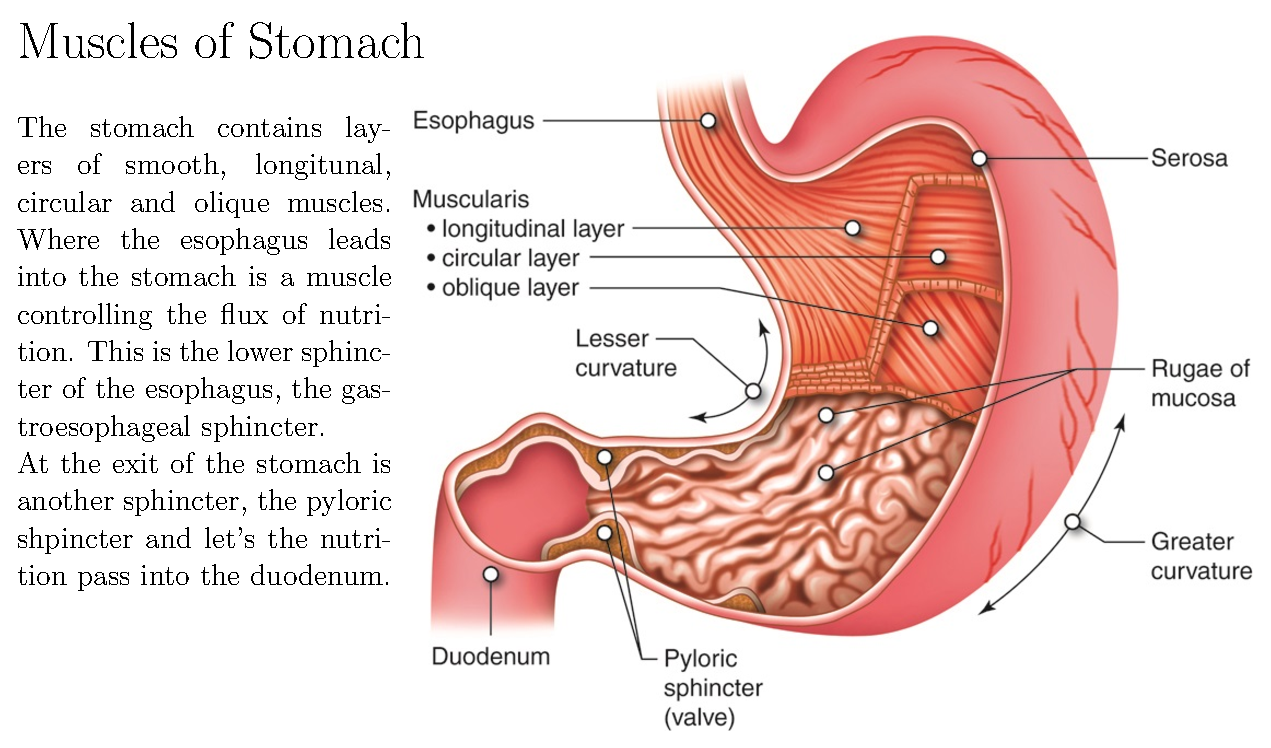
\includegraphics[width=12.5cm]{Stomach}
  \caption{The muscles of the stomach~\cite{Stomach}}\label{stomach}
\end{figure}

In the second digestive cavity, the stomach (figure \ref{stomach}),
hydrochloric acid -- chlorine and hydrogen ions -- disintegrate the pasta, shrimps and vegetables.
They open the cells of the plants, so that the vitamins\index{vitamins} get released.
The stomach contracts, mixing the whole thing up.

Around 50 tons of food and drinks pass through the stomach in a lifetime.
The enzymes of the stomach are doing hard work.
They split up long protein chains (for instance from the shrimps) into shorter
peptides\index{peptides} and into the smallest components, the amino acids\index{amino acids}.

\section{The Hunger Brake}

When the stomach is full, the I--am--saturated hormone cholecystokinin\index{cholecystokinin} signals the hypothalamus: ``Stop eating''.
If you eat more in that moment, the fat tissue produced leptin\index{leptin}.
This hormone goes over the blood stream into the brain and tells it: ``There's enough energy here''.
In people afflicted with overweight\index{symptom!overweight}, this doesn't work anymore.
Leptin is there, but the brain doesn't listen to it.


\begin{figure}[htb!]
  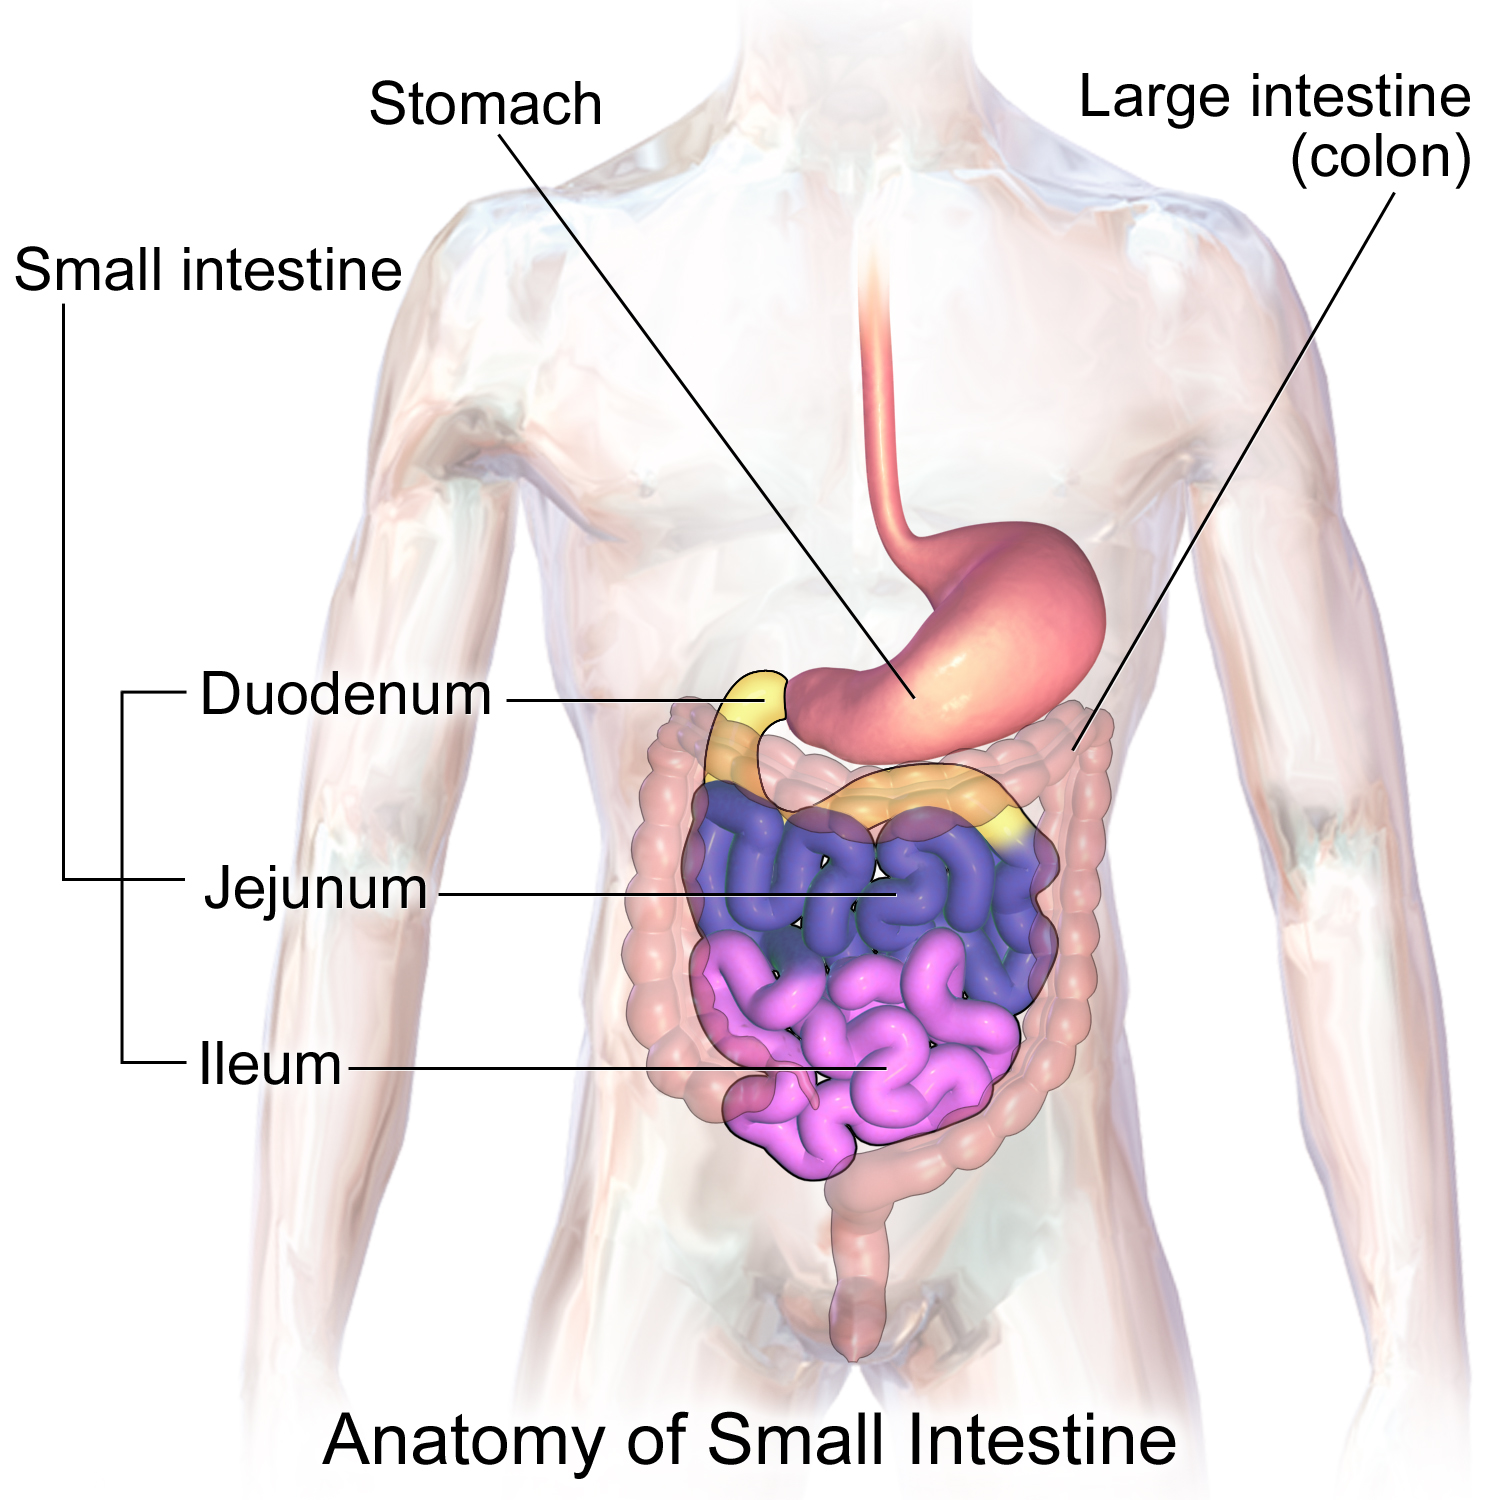
\includegraphics[width=12.5cm]{SmallIntestine}
  \caption{The small intestine and a cross section of it~\cite{SmallInt} and~\cite{LayersInt}}\label{SmallInt}
  \end{figure}


 
After two hours, the sphincter at the end of the stomach opens and sends a slurry into the small intestine\index{intestine!small}
(figure \ref{SmallInt} on page~\pageref{SmallInt}).
That's where it's decided what can go into the bloodstream.

\mytextbox[0]{
  \begin{description}
  \item[Cholecystokinin (CCK--1)] is a peptide hormone of the stomach -- intestine area.
    In the brain, it plays in important role as a neurotransmitter.
    A verbatim translation of the the name means gall bladder mover.
    \item[Leptin (Greek: lepto = thin)] is a hormone, which has been discovered 1994 by the molecular biologist Jeffrey Friedman.
      Leptin, which gets secreted by adipocytes (fat storage cells)\index{adipocyte} has the effect of inhibiting the appetite.
      Leptin plays an important role in the regulation of fat management and storage of mammals.
  \end{description}
}

\begin{figure}[htb!]
  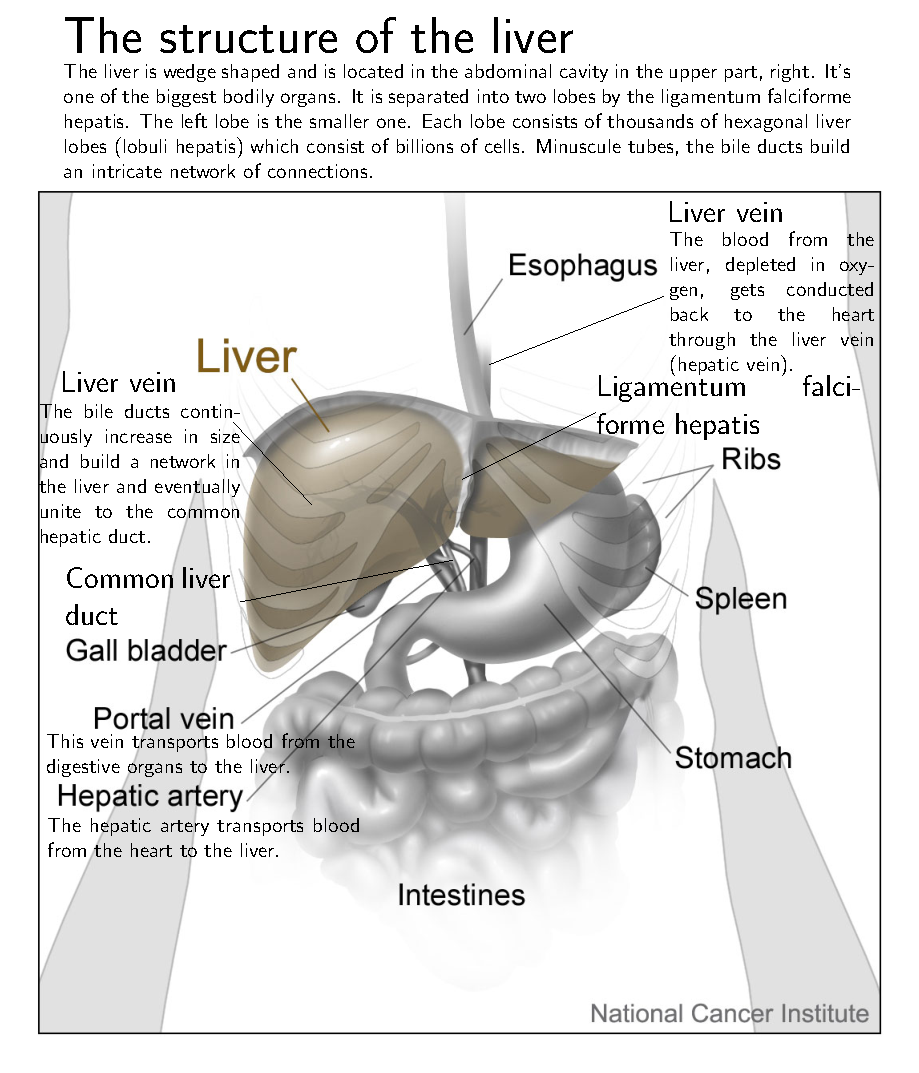
\includegraphics[width=12.5cm]{Liver}
  \caption{The liver and it's internal structure~\cite{Liver}}\label{liver}
  \end{figure}


  \section{That's how the Fat gets onto the Hips}

  \begin{figure}[htb!]
    \begin{center}
  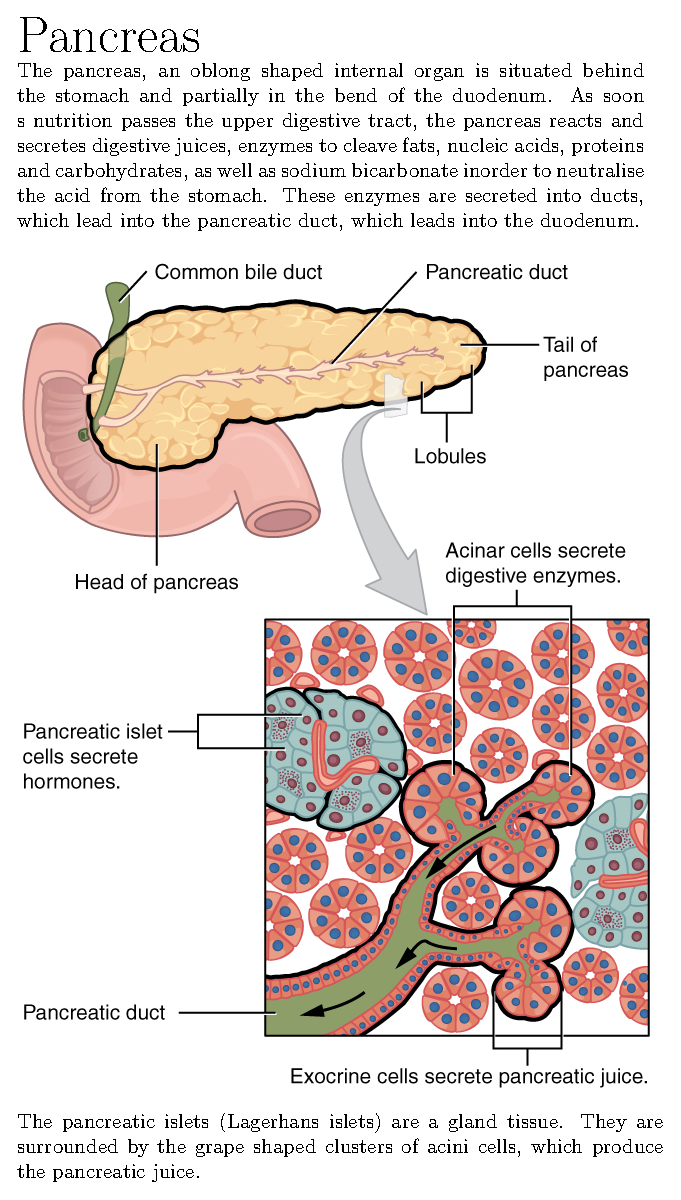
\includegraphics[width=8cm]{Pancreas}
  \caption{The pancreas~\cite{Pancreas2}}\label{pancreas}
  \end{center}
  \end{figure}

  \begin{figure}[htb!]
    \begin{center}
  \includegraphics[width=5cm]{Muscles}
  \caption{The muscular system~\cite{MusclesBougle}}\label{muscles}
  \end{center}
  \end{figure}

    \begin{figure}[htb!]
    \begin{center}
  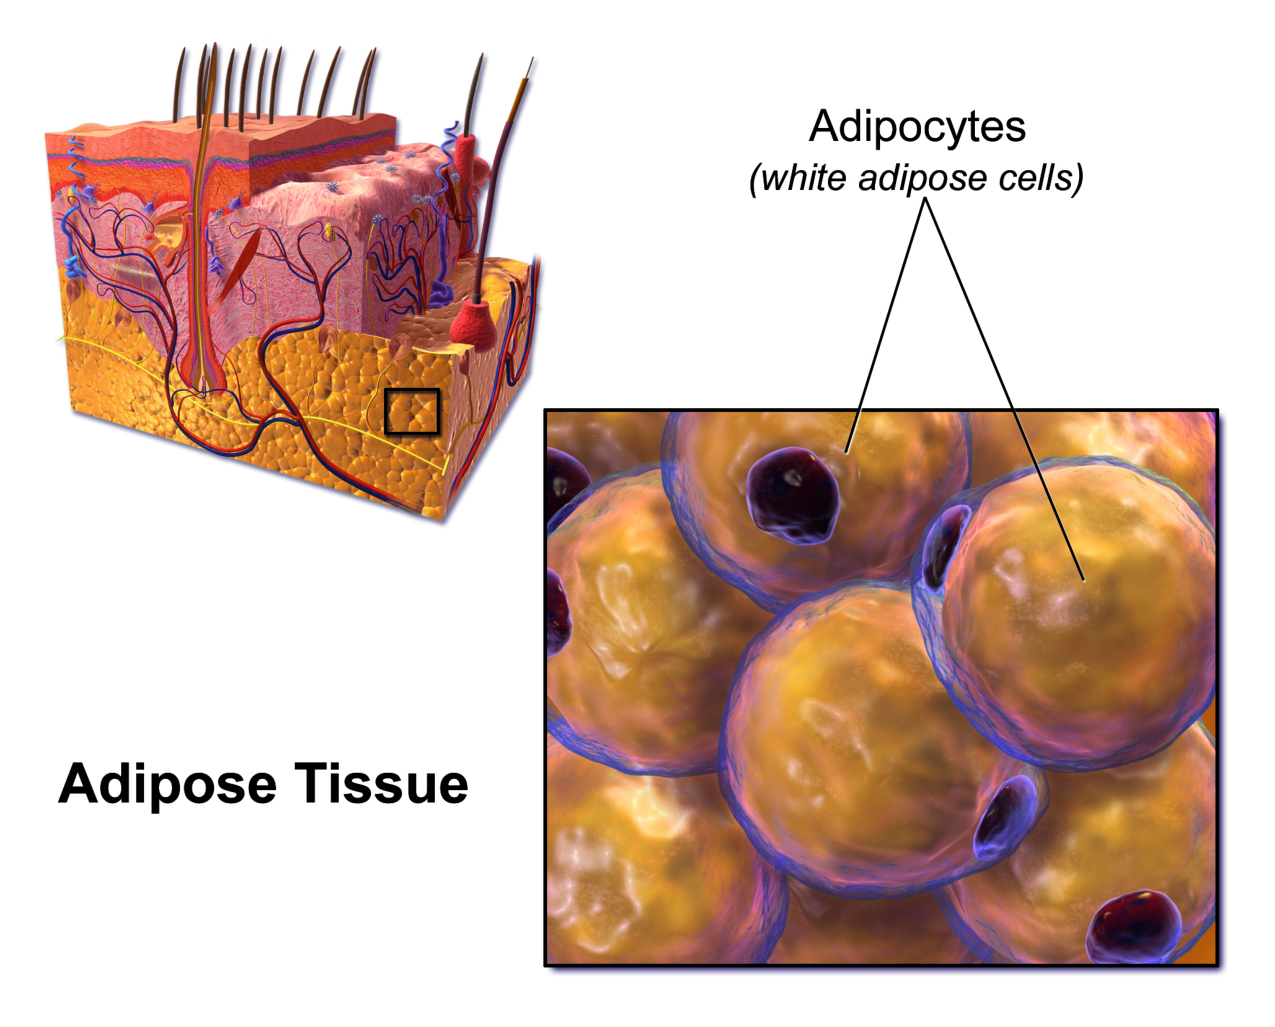
\includegraphics[width=9cm]{AdiposeTissue}
  \caption{Adipose Tissue~\cite{BlausenLimbic}}\label{adipose}
  \end{center}
  \end{figure}


As\index{metabolism!fat}\index{fat} soon as the slurry arrives, the gall\index{gall} (see liver in figure \ref{liver}) sends it's acidic juice.
Gall salts surround the fat globules and prepare them for the cleaving action of the enzymes from the pancreas\index{pancreas} (figure~\ref{pancreas}).
Lipases\index{lipase} cut fatty acids from the fat molecules.
In the cells of the colon, the fatty acids get packed into transport molecules, the so called chylomicrons\index{chylomicron}.
They carry the fat through the blood stream, making the blood milky with a white hue.
In the blood vessels, there are enzymes, which are waiting for these energy deliveries: lipo--protein lipases.
They suck the fat out from the protein package, and sends it to the muscles (figure~\ref{muscles})
to be burned, to rejuvenate the cell walls --- or to store it in the fat deposits.
In average, we have 20 billion fat cells\index{cell!fat} (figure~\ref{adipose}).
But they can reproduce and increase in number, very much not to our liking.
That can happen in childhood, but as studies showed, as well during the adult life.
And they can swell by a factor of a thousand, as if a pinhead would grow to the size of a golf ball.

\section[What Happens with Food?]{What Happens with Sugars, Proteins and Vital Substances?}

In the small intestine, enzymes cleave starch and sugar\index{metabolism!carbohydrates} into smaller molecules, fructose and glucose.
Sugar transporters brings them into the blood stream.
Accurate sensors continuously measure the level of sugar in the blood and transmit the data to the brain.
That mobilizes the pancreas to produce insulin\index{insulin}, which directs the excess of sugar into the cells.
Furthermore, the small intestine isolates vitamins, minerals and trace elements and sends them into the blood stream.\index{metabolism!vital substances}
From there, they get to their destination, the individual cells.
Calcium reinforces the bones, iron brings color into the blood, iodine goes to the thyroid gland in order to be used to build hormones.
The protein molecules get cleaved further\index{metabolism!protein} by enzymes
and specialized transport molecules bring the amino acids\index{amino acids} and protein fragments into the blood stream.
In the body, they get incorporated into the proteins of the body, into hormones, immune system, skin and hair.
Each of our 70 trillions of body cells will be reconstructed and repaired with the proteins from food.

But not all proteins are allowed to pass the intestinal barrier\index{intestinal barrier}: foreign proteins have to stay stay out of the blood.
Sometimes they nevertheless end up in our body and cause asthma and skin eczema.\index{symptom!asthma}\index{symptom!skin eczema}
Nobody knows why that is the cause and that question also is being researched.
But what is certain is that our intestine is our biggest immune system.
And that has the be cared for, by providing it with nutrition that our body knows.

\section{Final Stop: the Large Intestine}

    \begin{figure}[htb!]
    \begin{center}
  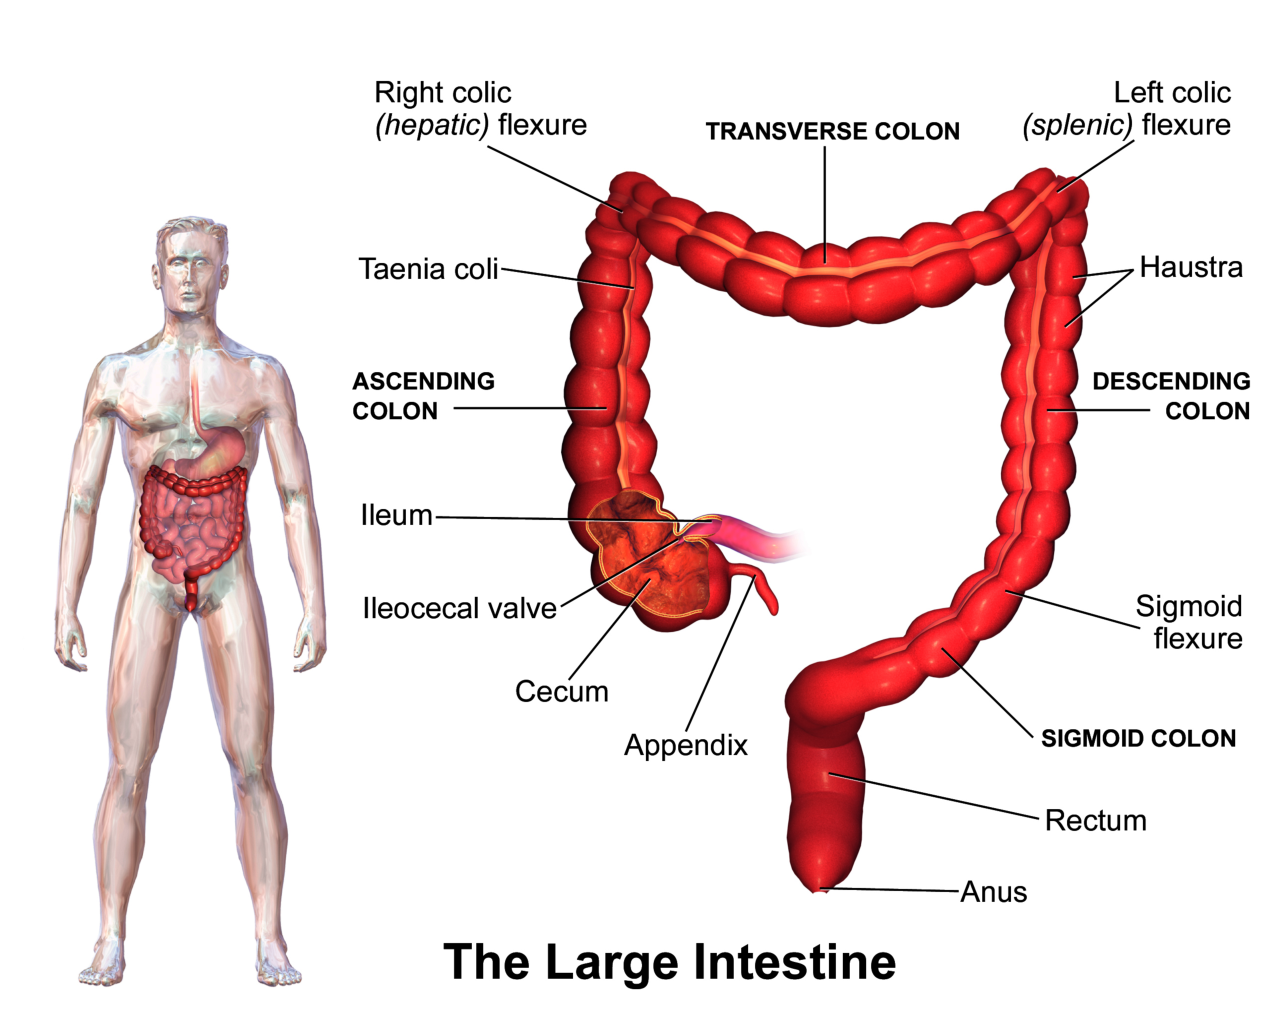
\includegraphics[width=9cm]{LargeIntestine}
  \caption{The large intestine~\cite{BlausenLimbic}}\label{LargeIntestine}
  \end{center}
  \end{figure}


  Two things continue on into the large intestine\index{intestine!large} (figure~\ref{LargeIntestine}):
  a part of the water and indigestible fibers\index{metabolism!fibers} of veggies and grains. 
Toxins and cholesterol are getting dragged along for sewer system.
The large intestine thickens it up by removing water from it.
The large intestine is a gigantic ecosystem in itself.
In one drop of intestinal fluids are billions of bacteria.
They are going at the indigestible fiber walls and deliver fatty acids to the large intestine
and release defensive weapons against cancer,\index{symptom!cancer} for instance flavanoids\index{flavanoids} from the fibers.
They produce the well known gases as a byproduct of processing of fibers.
The fibers shorten the time of the reminders in the colon.
It urges us to have a daily bowel movement.
That way the remainders find their natural end.


\end{document}